\documentclass[a4,12pt]{article}

\usepackage{amsmath, amsthm, amssymb, amsfonts}
\usepackage[utf8]{inputenc}
\usepackage[T1]{fontenc}
\usepackage[slovene]{babel}
\usepackage{thmtools}
\usepackage{lmodern}
\usepackage[colorlinks=false]{hyperref}
\usepackage{textcomp}

\usepackage{floatrow}
\usepackage{wrapfig}

\usepackage{graphicx}
\usepackage{tikz}
\usepackage{tkz-euclide}
\usepackage{setspace}
\usepackage{geometry}
\usepackage{float}
\usepackage{framed}

% \usepackage[dvipsnames]{xcolor}
\usepackage[theorems]{tcolorbox}

\newtcbtheorem[number within=section]{definition}{Definicija}
{colback=green!5,colframe=green!35!black,fonttitle=\bfseries}{th}

\newtcbtheorem[use counter from=definition, number within=section]{note}{Opomba}
{colback=yellow!5,colframe=yellow!35!black,fonttitle=\bfseries}{th}

\newtcolorbox[auto counter,number within=section]{example}{
colback=orange!5!white,colframe=orange!75!black,fonttitle=\bfseries,
title=Primer}


% gensymb is currently broken, so we use this workaround
\newcommand{\degree}{^\circ}
\newcommand{\R}{\mathbb{R}}


\title{Zapiski s predavanj iz algebre 1}

\begin{document}
\maketitle

\tableofcontents

\section{Vektorji v \(\R^3\)}
\subsection{Koordinatni sistem}
    Model za realna števila je \textbf{realna os}: premica, na kateri označimo točki \(0\) -- izhodišče in \(1\) -- enoto.
    Običajno je \(1\) desno od \(0\). Na ta način smo v premico vpeljali koordinatni sistem. Vsakemu realnemu števil
    ustreza natanko ena točka na realni osi.

    Če je \(x > 0\), potem številu \(x\) ustreza točka desno od \(0\), ki je za \(x\) oddaljena od \(0\). Če je 
    \(x < 0\), številu \(x\) ustreza točka levo od \(0\), ki je za \(-x\) oddaljena od \(0\).
    Obratno tudi velja: Vsaki točki na realni osi ustreza natanko eno realno število.
    Imamo torej bijekcijo med \(\R\) in realno osjo.

    \[\R^2 = \R \times \R = \left\{\left(x, y\right); x \in \R, y \in \R\right\}\]
    Model za \(\R^2\) je \textbf{ravnina} z danim koordinatnim sistemom. Običajno uporabljamo pravokotni koordinatni sistem.
    Sestavljata ga pravokotni realni osi, ki se sekata v točki \(0\) -- izhodišču obeh realnih osi. Običajno je ena realna
    os vodoravna in kaže desno, druga pa navpična in kaže gor. Vodoravna se imenuje \textbf{abscisna} os, navpična pa
    \textbf{ordinatna} os.

    {
        Izberimo točko \(T\) v ravnini. Vzporednica ordinatni osi, ki poteka skozi \(T\), seka abscisno os v natanko eni
        točki \(x\). Vzporednica abscisni osi, ki poteka skozi točko \(T\), seka ordinatno os v natanko eni točki \(y\).
        Točki \(T\) smo priredili urejen par števil \(\left(x, y\right) \in \R^2\). Točko označimo \(T\left(x, y\right)\)
        in pravimo, da sta \(x\) in \(y\) koordinati točke \(T\). To prirejanje je injektivno, saj če bi za eno točko našli
        več možnih koordinat, bi pomenilo, da je na več vzporednicah, kar pa ne more biti res. Velja tudi surjektivnost,
        iz tega dvojega pa sledi tudi bijektivnost.
        \begin{figure}[H]
            \centering
            \begin{tikzpicture}[scale=0.50]
                % koordinatni sistem
                \draw[-stealth] (-3, 0) -- (3, 0);
                % \node at (3, 0) [below] {\(x\)};
                \draw[-stealth] (0, -3) -- (0, 3);
                % \node at (0, 3) [left] {\(y\)};
                
                % točka, vzporednici
                \coordinate[label = above right:$T$] (T) at (2, 2);
                \node at (T) [circle,fill,scale=0.2] {\(T\)};
                \draw[dashed] (2, 2) -- (2, 0);
                \draw[dashed] (2, 2) -- (0, 2);
                \node at (2, 0) [below] {\(x\)};
                \node at (0, 2) [left] {\(y\)};
            \end{tikzpicture}
        \end{figure}
    }

    Dobili smo preslikavo iz ravnine v \(\R^2\), ki je bijekcija, zato bomo množico \(\R^2\) identificirali
    z ravnino z danim koordinatnim sistemom.
    
    \begin{definition}{Razdalja med točkama}{def:razdalja}
        \emph{Razdalja} med točkama \(T_1\left(x_1, y_1\right)\) in \(T_2\left(x_2, y_2\right)\) je definirana s predpisom:
        \[d\left(T_1, T_2\right) = \sqrt{\left(x_1 - x_2\right) ^ 2 + \left(y_1 - y_2\right)^2}\]
        \begin{figure}[H]
            \centering
            \begin{tikzpicture}
                \coordinate (A) at (0, 0);
                \coordinate (B) at (3, 2);
                \filldraw[black] (A) circle (2pt) node[anchor=east]{\(T_1\)};
                \filldraw[black] (B) circle (2pt) node[anchor=west]{\(T_2\)};
                \draw[dashed] (A) -- (3, 0);
                \draw[dashed] (B) -- (3, 0);
                \draw (B) -- (A);
                \node at (3, 1) [right] {\(y_2 - y_1\)};
                \node at (1.5, 0) [below] {\(x_2 - x_1\)};
            \end{tikzpicture}
        \end{figure}
    \end{definition}

    \noindent \(\R^3 = \R \times \R \times \R = \left\{\left(x, y, z\right); x,y,z \in \R\right\}\)
    Model za \(\R^3\) je \textbf{prostor} z danim koordinatnim sistemom. Sestavljajo ga tri realne osi, ki
    so paroma pravokotne in se sekajo v natanko eni točki, ki je izhodišče na vseh treh realnih oseh.

    Dogovorimo se, da uporabljamo pozitivno orientiran koordinatni sistem: če se postavimo v enoto na \(z\)-osi in
    pogledamo ravnino, določeno z osema \(x\) in \(y\), potem vidimo koordinatni sistem, ki smo ga definirali za \(\R^2\). To pomeni:
    os \(x\) zavrtimo v pozitivni smeri (\(\circlearrowleft\) -- nasprotni smeri urinega kazalca) za \(90 \degree\), da dobimo os \(y\).
    Pomagamo si s pravilom desnega vijaka. \url{https://xkcd.com/199/}

    Vsaki trojici \(\left(x, y, z\right) \in \R^3\) lahko priredimo točko \(T\left(x, y, z\right)\) v prostoru.
    \(x\), \(y\) in \(z\) so koordinate točke \(T\).
    Preslikava, ki trojici \((x, y, z) \in \R^3\) priredi \(T\left(x, y, z\right)\) je bijekcija.
    Inverz: naredimo vzporednico \(z\) osi -- seka ravnino \(xy\) v 1 točki \(T'\). Vzporednica skozi 
    \(T\) na daljico \(0T'\) seka \(z\) os v natanko eni točki \(z\). Koordinati točke \(T'\) že 
    znamo poiskati, to sta \(x\) in \(y\) koordinati točke \(T\).

    \textbf{Razdalja} med točkama \(T_1\left(x_1, y_1, z_1\right)\) in \(T_2\left(x_2, y_2, z_2\right)\) je definirana s predpisom:
    \[d\left(T_1, T_2\right) = \sqrt{{\left(x_1 - x_2\right)}^2 + {\left(y_1 - y_2\right)}^2 + {\left(z_1 - z_2\right)}^2}\]

    Na \(\R^3\) definiramo operaciji: \begin{itemize}
        \item seštevanje: \(\left(x_1, y_1, z_1\right) + \left(x_2, y_2, z_2\right) = \left(x_1 + x_2, y_1 + y_2, z_1 + z_2\right)\)
        \item množenje s skalarjem: \(\lambda \cdot \left(x, y, z\right) = \left(\lambda x, \lambda y, \lambda z\right)\)
    \end{itemize}

\subsection{Vektorji}
    \begin{definition}{Krajevni vektor}{def:krajevni_vektor}
        Naj bo \(a = \left(x, y, z\right)\) poljubna točka. \emph{Krajevni vektor} točke \(a\) je usmerjena daljica od \(0\) do \(a\).
        Označimo ga z \(\vec{a} = \left(x, y, z\right)\).

        Oznaka \(\left(x, y, z\right)\) za krajevni vektor je ista kot oznaka za končno točko \(x, y, z\).
        Vsakemu krajevnemu vektorju pripada natanko ena končna točka in vsaki točki v prostoru pripada natanko en krajevni vektor, ki
        ima to točko za končno točko. Torej imamo bijekcijo med \(\R^3\) in množico krajevnih vektorjev.
    \end{definition}
    \begin{definition}{Vektor}{def:vektor}
        \emph{Vektor} \(\vec{a} = \left(x, y, z\right)\) je množica vseh usmerjenih daljic, ki jih dobimo tako, da krajevni vektor \(\vec{a}\)
        vzporedno premaknemo
    \end{definition}
    \begin{note}{Pogosto bomo uporabljali nenatančno definicijo vektorja}{note:nenatancno_vektor}
        Vektor je določen z usmerjeno daljico. Dva vektorja sta enaka, če sta pripadajoči usmerjeni daljici
        vzporedni, enako dolgi in kažeta v isto smer.
    \end{note}
    \begin{note}{}{note:ekv}
        Ko bomo delali relacije, bomo videli, da je vektor ekvivalenčni razred za
        relacijo, da sta dve usmerjeni daljici vzporedni, enako dolgi in kažeta v isto smer.
    \end{note}

    \noindent Če je vektor določen z usmerjeno daljico od točke \(A\) do točke \(B\), ga bomo označevali z \(\overrightarrow{AB}\).

    Med množico vektorjev in množico krajevnih vektorjev imamo bijekcijo: vektorju priredimo krajevni vektor, ki je usmerjena daljica
    iz vektorja in ima začetek v koordinatnem izhodišču. Imamo bijekcijo med \(\R^3\) in množico vektorjev.

    Na \(\R^3\) smo imeli operaciji seštevanje in množenje s skalarjem. Na množici vektorjev definiramo operaciji skladno s temi operacijami.

    \begin{definition}{Seštevanje vektorjev}{def:sestevanje_vektorjev}
        \(\left(x_1, y_1, z_1\right) + \left(x_2, y_2, z_2\right) = \left(x_1 + x_2, y_1 + y_2, z_1 + z_2\right)\).
        Lahko je razmisliti, da je tak način seštevanja dobro definiran kjerkoli v prostoru.
        \begin{figure}[H]
            \centering
            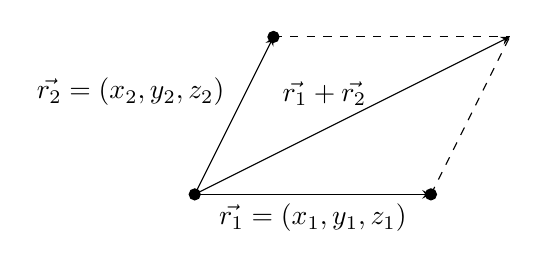
\begin{tikzpicture}
                \coordinate (O) at (0, 0);
                \coordinate (A) at (3, 0);
                \coordinate (B) at (1, 2);
                \filldraw[black] (A) circle (2pt) node[anchor=east]{};
                \filldraw[black] (B) circle (2pt) node[anchor=west]{};
                \filldraw[black] (O) circle (2pt) node[anchor=south]{};
                \draw[dashed] (A) -- (4, 2);
                \draw[dashed] (B) -- (4, 2);
                \draw[-stealth] (O) -- (A);
                \draw[-stealth] (O) -- (B);
                \draw[-stealth] (O) -- (4, 2);
                \node at (2, 1) [above, xshift=-10] {\(\vec{r_1} + \vec{r_2}\)};
                \node at (1.5, 0) [below] {\(\vec{r_1} = \left(x_1, y_1, z_1\right)\)};
                \node at (0.5, 1) [above left] {\(\vec{r_2} = \left(x_2, y_2, z_2\right)\)};
            \end{tikzpicture}
        \end{figure}
    \end{definition}
    \begin{definition}{Ničelni vektor}{def:nicelni_vektor}
        Vektor \(\vec{0} = \left(0, 0, 0\right)\) imenujemo \emph{ničelni vektor}. Določen je z vsako usmerjeno daljico,
        ki ima začetek in konec v isti točki. Velja \(\vec{a} + \vec{0} = \vec{a}\) za vsak vektor \(\vec{a} \in \R^3\).
    \end{definition}
    \begin{definition}{Nasprotni vektor}{def:nasprotni_vektor}
        \emph{Nasprotni vektor} vektorja \(\vec{a} = \left(x, y, z\right)\) je vektor \(-\vec{a} = \left(-x, -y, -z\right)\).
        Če je \(\vec{a}\) določen z usmerjeno daljico od \(A\) do \(B\), je \(-\vec{a}\) določen z usmerjeno daljico od \(B\) do \(A\).
        Velja \(\vec{a} + \left(-\vec{a}\right) = \vec{0}\) za vsak vektor \(\vec{a} \in \R^3\).
    \end{definition}
    \begin{definition}{Odštevanje vektorejev}{def:odstevanje_vektorjev}
        \(\vec{a} - \vec{b} = \vec{a} + \left(-\vec{b}\right)\)
        \begin{figure}[H]
            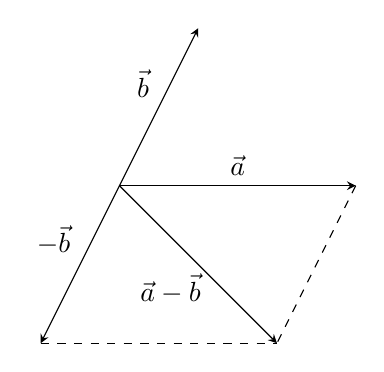
\begin{tikzpicture}
                \draw[-stealth] (0, 0) -- (3, 0);
                \draw[-stealth] (0, 0) -- (1, 2);
                \node at (0.5, 1) [above left] {\(\vec{b}\)};
                \node at (1.5, 0) [above] {\(\vec{a}\)};
                \draw[-stealth] (0, 0) -- (2, -2);
                \node at (1, -1) [below, xshift=-10pt] {\(\vec{a}-\vec{b}\)};
                \draw[dashed] (3, 0) -- (2, -2);
                \draw[-stealth] (0, 0) -- (-1, -2);
                \node at (-0.5, -1) [above left] {\(-\vec{b}\)};
                \draw[dashed] (-1, -2) -- (2, -2);
            \end{tikzpicture}
        \end{figure}
    \end{definition}
    \begin{definition}{Množenje vektorja s skalarjem}{def:mnozenje_vektorja_s_skalarjem}
        \(\lambda \cdot \left(x, y, z\right) = \left(\lambda x, \lambda y, \lambda z\right)\)
        \begin{figure}[H]
            \begin{tikzpicture}
                \filldraw[black] (0, 0) circle (2pt) node{};
                \draw[-stealth] (0, 0) -- (3, 0.5);
                \node at (1.5, 0.25) [above] {\(\vec{a}\)};
                \draw[-stealth] (0, 0) -- (6, 1);
                \node at (4.5, 0.75) [above] {\(2\vec{a}\)};
                \draw[-stealth] (0, 0) -- (-3, -0.5);
                \node at (-1.5, -0.25) [above] {\(-\vec{a}\)};
            \end{tikzpicture}
        \end{figure}
    \end{definition}

    \noindent Lastnosti:
    \begin{enumerate}
        \item \(\left(\vec{a} + \vec{b}\right) + \vec{c} = \vec{a} + \left(\vec{b} + \vec{c}\right)\) asociativnost
        \item \(\vec{a} + \vec{0} = \vec{a}\)
        \item \(\vec{a} + \left(- \vec{a}\right) = \vec{0}\)
        \item \(\vec{a} + \vec{b} = \vec{b} + \vec{a}\) komutativnost
        \item \(r \cdot \left(\vec{a} + \vec{b}\right) = r \cdot \vec{a} + r \cdot \vec{b}\) distributivnost
        \item \(\left(r + s\right) \cdot \vec{a} = r \cdot \vec{a} + s \cdot \vec{a}\) distributivnost
        \item \(\left(r \cdot s\right) \cdot \vec{a} = r \cdot \left(s \cdot \vec{a}\right)\)
        \item \(1 \cdot \vec{a} = \vec{a}\)
    \end{enumerate}
    Dokaz za vse te lastnosti dobimo, če razpišemo vektorje po komponentah. Kasneje bomo videli,
    da je z aksiomi od 1 do 8 definiran vektorski prostor.

    \begin{definition}{Linearna kombinacija vektorjev}{def:linearna_kombinacija_vektorjev}
        Naj bodo \(\vec{a_1}, \vec{a_2}, \ldots, \vec{a_n}\) poljubni vektorji. Vsak vektor oblike
        \(\alpha_1 \vec{a_1} + \alpha_2 \vec{a_2} + \ldots + \alpha_n \vec{a_n}\), kjer so \(\alpha_1, \alpha_2, \ldots, \alpha_n \in \R\),
        imenujemo linearna kombinacija vektorjev \(\vec{a_1}, \vec{a_2}, \ldots, \vec{a_n}\).
        \begin{example}
            \(2\vec{a_1} + \frac{3}{2} \vec{a_2} - \vec{a_3}\) je linearna kombinacija vektorjev \(\vec{a_1}, \vec{a_2}, \vec{a_3}\).
        \end{example}
    \end{definition}
\end{document}